\documentclass[../Article_Model_Parameters.tex]{subfiles}
\graphicspath{{\subfix{../Figures/}}}
\begin{document}
	
	\subsubsection{Concentration limit}
	
	To mimic that not all solute might be obtained at specific operating conditions, the coefficient $\gamma$ is introduced to limit the available oil. The $\gamma(c_s)$ describe the reverse logistic function, which is equal to unity above the $c_{lim}$, the saturation concentration, and equal to zero, below the $c_{lim}$. The $\gamma$ parameter multiply the solute concentration term in solid phase in the concentration gradient. As the concentration of solute decrease, it can reach the limiting value $c_{lim}$ when the $\gamma$ goes to zero and stop the extraction from the solid.
	The $\gamma(c_f)$ for $c_{sat}=5$ is shown on figure \ref{fig: Gamma_function}.
			
	{\footnotesize
		\begin{equation}
			\gamma(c_s) = \cfrac{1}{1+\exp ( -k_{sat} \left( c_s - c_{lim} \right) ) }
			\label{EQ: C_sat_function}
			\end{equation}
	}
			
	where $k_{lim}$ describe the curvature of the $\gamma$ function, and it is defined as $k_{lim} = 1$. The bigger value of the $k_{sat}$ the steeper the function is. In the limit when $ k_{lim}\rightarrow+\infty$ become a step function. If the growth rate is to high, the gradient of the $\gamma$ function become high, or goes to infinity, which might cause difficulties for a gradient-based optimizer.
			
	\begin{figure}[h!]
		\centering
			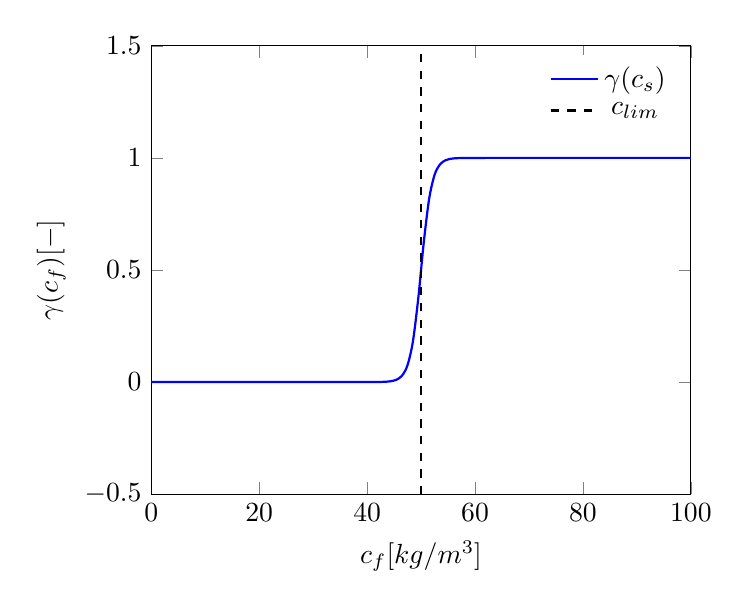
\begin{tikzpicture}
					
				\begin{axis}[
					legend style={draw=none},
					xmin = 0, xmax = 100,
					ymin = -0.5, ymax = 1.5,
					xlabel = {$c_f[kg/m^3]$},
					ylabel = {$\gamma(c_f)[-]$}]
					\addplot[
					domain = 0:100,
					samples = 100,
					smooth,
					thick,
					blue,
					] { 1 / (1 + exp( 1 * ( 50 - x ) ) ) };
					\addplot[thick, samples=50, dashed, domain=0:1.5, black] coordinates {(50,-0.5)(50,1.5)};
					
					\addlegendentry{$\gamma(c_s)$}
					\addlegendentry{$c_{lim}$}
				\end{axis}
					
			\end{tikzpicture}
			\caption{$\gamma(c_s)$ function under assumption of $c_{lim}=50~[kg/m^3]$}
			\label{fig: Gamma_function}
	\end{figure}
			
			
	The final form of the extraction kinetic equation is given by equation \ref{Model_kinetic}.
			
	{\footnotesize
		\begin{equation}
			\label{Model_kinetic}
				{\color{blue}r_e}(t,z) = -\cfrac{{\color{orange}D_i}({\color{blue}T}(t,z), {\color{red}P}(t))}{{\color{magenta} \mu l^2} } \left({\color{blue}c_s}(t,z) \gamma(c_s) - \cfrac{{\color{magenta}\rho_s}}{{\color{orange}k_m}({\color{blue}T}(t,z)){\color{orange}\rho}({\color{blue}T}(t,z),{\color{red}P}(t))}  {\color{blue}c_f}(t,z) \right)
		\end{equation} }
			
\end{document}